\section{Tareas y mensajes}

\subsection{Envío de un mensaje}
\label{ssec:envio_mensaje}

El envío de un mensaje comprende todo el recorrido desde que un usuario crea y envía un mensaje desde su pantalla de feed hasta que este llega al resto de usuarios asociados, se corresponde con el \nameref{sec:cu:mensajes} y se puede ver en la \fref{dia:secuencia_envio_mensaje}.

\begin{figure}[H]
    \centering
    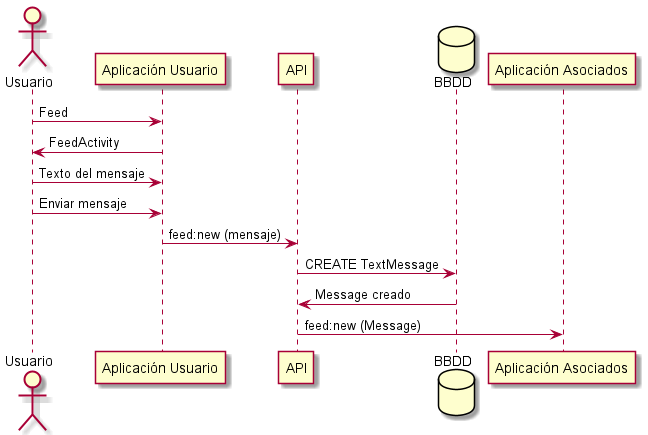
\includegraphics[width=0.65\textwidth]{images/Diseño/SecuenciaEnviarMensaje.png}
    \caption{Diagrama de secuencia del envío de un mensaje}
    \label{dia:secuencia_envio_mensaje}
\end{figure}

La secuencia de envío de mensajes arranca cuando un usuario redacta un mensaje y utiliza el botón de enviar de la actividad del feed. Al hacerlo, la aplicación envía el mensaje a través del socket según el evento del \fref{ws:feed_send}. Cuando la \acrshort{api} recibe dicho mensaje lo persiste en la base de datos y lo reenvía por medio del mismo evento al resto de usuarios asociados, que lo mostrará en pantalla si están conectados a la sala de feed.

\subsection{Creación de nueva tarea}

Una nueva tarea (\nameref{sec:cu:tareas}) se puede crear de dos maneras distintas. Una por medio del envío de la misma a través del feed, esta vía sigue un proceso similar al envío de mensajes, únicamente cambiando el tipo de entidad que se persiste, véase pues la sección anterior (\ref{ssec:envio_mensaje} \nameref{ssec:envio_mensaje}). La otra es desde la pantalla de tareas por medio de la función de crear una nueva tarea.

\begin{figure}[H]
    \centering
    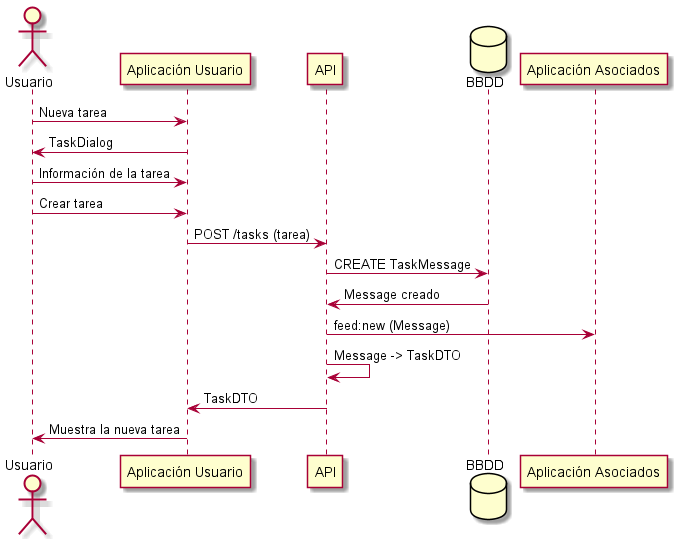
\includegraphics[width=0.75\textwidth]{images/Diseño/SecuenciaCrearTarea.png}
    \caption{Diagrama de secuencia de la creación de una tarea}
    \label{dia:secuencia_creacion_tarea}
\end{figure}

En el diálogo desplegado por dicha opción de la pantalla de tareas el usuario rellenará los datos de la tarea y una vez confirme su creación, la aplicación móvil enviará dicha tarea a la \acrshort{api} por medio del \gls{endpoint} del \fref{api:crear_tarea}. Una vez la \acrshort{api} reciba dicha tarea la enviará a la base de datos para persistirla y completar su creación con una ID (ver \ref{ssec:estado_tarea} \nameref{ssec:estado_tarea}). Finalmente, la tarea obtenida tras dicha creación será enviada a través de dos canales: primero como mensaje por WebSocket a la sala del feed (\fref{ws:feed_send}) y, posteriormente, como respuesta a la petición \acrshort{http} como \nameref{dto:taskmessage}.

\subsection{Estado de una tarea}
\label{ssec:estado_tarea}

Las cuatro acciones que se pueden realizar sobre una tarea (crearla, marcarla como hecha, marcarla como no hecha y eliminarla) derivan en los estados que se pueden ver en la \fref{dia:estado_tarea}. Primero, cuando un usuario crea una nueva tarea desde su aplicación esta existe inicialmente como \textbf{Nueva} y contiene los datos de un \nameref{dto:taskmin}. 

Esta tarea es enviada por la aplicación por medio de cualquiera de los dos sistemas de creación (WebSocket o \acrshort{http}). Entonces es recibida por la \acrshort{api} y persistida en la base de datos, momento en el que recibe una ID y se convierte en \textbf{Creada}. A diferencia de una tarea Nueva, que siempre existe como \emph{No hecha}, una tarea Creada puede tener dos estados: \textbf{Hecha}, en caso de que haya sido completada, y \emph{No hecha}, si aún se debe realizar. La transición entre estos dos estados pasa por peticiones a los \glspl{endpoint} respectivos (\fref{api:marcar_tarea_hecha} \nameref{api:marcar_tarea_hecha} y \fref{api:marcar_tarea_no_hecha} \nameref{api:marcar_tarea_no_hecha}) con la ID de la tarea.

\begin{figure}[H]
    \centering
    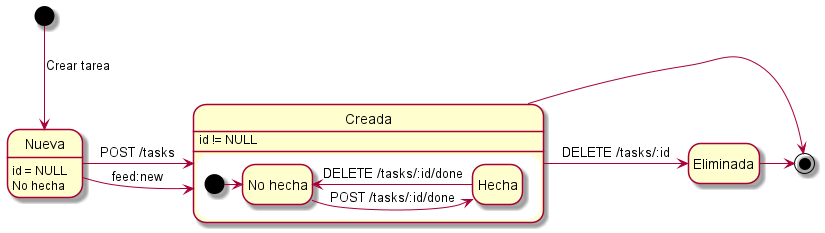
\includegraphics[width=0.75\textwidth]{images/Diseño/EstadoTarea.png}
    \caption{Diagrama de estado de una tarea}
    \label{dia:estado_tarea}
\end{figure}

Finalmente, el último estado que puede tomar una tarea es el de \textbf{Eliminada}, para ello la tarea debía estar ya Creada y una petición de eliminación (véase \nameref{api:eliminar_tarea}) debe haber sido enviada a la \acrshort{api}. Tanto Creada como Eliminada son estados finales de la tarea, el único estado inicial es el de Nueva.